\documentclass[]{article}
\usepackage{graphicx}
\usepackage[utf8]{inputenc}
\usepackage{cite}
\usepackage{amsmath,amssymb,amsfonts}
\usepackage{textcomp}
\usepackage{xcolor}

\newcommand{\etal}{\textit{et al}}

\graphicspath{ {.} }

\begin{document}

\title{ECE598LV Lecture 25: Explainability I}
\author{
Zong Fan \\ BIOE, UIUC\\
zongfan2@illinois.edu
\and
Xiaobai Li \\ ECE, UIUC \\
xiaobai2@illinois.educommuist
}
\date{April 26, 2022}

\maketitle

\section{Interpretability of AI models}
\subsection{Why do we need to interpret?}
\begin{itemize}
\item \textbf{Artistic domains enable respect for human autonomy} 
\item \textbf{As part of creative conversation, some "theory of mind" of partner helps.}
\item \textbf{Build trust for users. (eg: Industry practitioners)}\\
Many times, the model itself is just a black box that can provide an output, which users will not understand unless they have an understanding of the knowledge in machine learning field. Therefore, if we can interpret the model, they can understand the model based on the interpretation and thus trust the model more because they understand it \cite{b8, b9}.
\item \textbf{Error correction(diagnosis)}\\
It's very likely that the model we built will have some sort of flaw or error that is not easy to debug directly. Interpret the model will help us understand what the model is trying to present and where is the model is looking at, thus making us understand the model designing process better thus allow us to find out the mistake that the model has in the process, enabling us to correct the error of the model\cite{b8,b9}.
\item \textbf{Help human designers of AI models to build better models.}\\
Many times people are just trying to play with hyperparameters randomly to improve performance, which might not work most of the time, and even if it works, we don't understand why it works. Using interpretability, we can interpret the model performance and behavior, and we might be able to find out which part of the process has room to improve, thus adjusting our model related to that part to build better models.
\item \textbf{Knowledge discovery (Music, Physics, etc)}\\
People and machine learning models are not always looking at the same thing when doing identical task. We can interpret the model and understand what the model is looking at, and the particular feature or structure that the machine learning model is looking at might provide new insight to us humans in that area and we might be able to discover new knowledge in that area. 
\item \textbf{Ask better question}\\
With better understanding of the model, we could raise better questions in the area, sort of similar to knowledge discovery and build a better model.
\item \textbf{Reasoning about failure mode}\\
With the process of interpreting the model, we could understand how the model works and why the model fails to work properly in some cases, and get the reason for the failure mode. Such knowledge will help us to avoid failure in the future.
\item \textbf{Support bias mitigation}\\
There are different kinds of biases that could be involved in the generative models. Interpreting the model will have us understand what kind of bias our model may have thus having better social responsibility.
\item \textbf{Control/influence the generative process}\\
We can use the outcome of the interpreted model to control the generative process, making the generative model output better.
\end{itemize}

\subsection{What could we interpret?}
\begin{itemize}
\item \textbf{Model focused}:\\
Explanation of input to output mapping (how do given setting lead to given output?) \cite{b14}
\item \textbf{Artifact itself}: \\
Putative algorithm that generated it that is human-interpretable \cite{b14}
\item \textbf{Internal representation}:\\
There are a lot of techniques and methods that will use latent space, so it's important to understand what the latent space is representing(nature of latent space). 
\item\textbf{Feature characterization(AI safety)}: \\
\end{itemize}


\subsection{How can we interpret the model?}
\begin{itemize}
\item {Assertion of properties (axiomatic)} 

\item {Human subject experiment} 
Use some techniques to ask people how well they understand. This is a technique that is widely used in psychology, social understanding and human-AI understanding.
\end{itemize}

\section{Examples of generative model interpretability} 
\subsection{BERTology} 
\subsubsection{Background: BERT}
BERT\cite{b10} is a transformer-based language model which won the best paper award in NAACL 2019, and there are over 150 studies that are surveyed on BERT\cite{b11}.

BERT’s key technical innovation is applying the bidirectional training of Transformer, a popular attention model, to language modelling. BERT makes use of Transformer, an attention mechanism that learns contextual relations between words (or sub-words) in a text. In its vanilla form, Transformer includes two separate mechanisms — an encoder that reads the text input and a decoder that produces a prediction for the task. Since BERT’s goal is to generate a language model, only the encoder mechanism is necessary.As opposed to directional models, which read the text input sequentially (left-to-right or right-to-left), the Transformer encoder reads the entire sequence of words at once. Therefore it is considered bidirectional, though it would be more accurate to say that it’s non-directional. This characteristic allows the model to learn the context of a word based on all of its surroundings (left and right of the word).\cite{b11}

BERTology is pretty much an interpretation of BERT to understand how BERT works. It's is a growing field of study concerned with investigating the inner working of large-scale transformers like BERT\cite{b12} There are multiple takeaways of BERT is discussed in BERTology. 

One of the main BERT takeaways is that if you look for linguistic information in BERT, you will probably find it. For example, BERT will prefer correct to incorrect Verb forms. Also, it's possible to learn a linear transformation of BERT vector space that corresponds to syntactic trees and has a lot of factual knowledge. 

Another main takeaway of BERT is that despite BERT having all the linguistic information, it does not seem to use all those information. This can be learned since BERT does not change prediction given different input perturbations. Bert can not reason over the fact it knows. For example, if we say a man walks into a house, we can know that the house is larger than the man, but BERT can not learn that since it goes beyond the fact that it knows. 

Issues with probing are also a takeaway for BERT. BERT embedding contains at least information of part of speech and syntactic chucks and roles. The problem with probing is that if the model did not observe some feature, that doesn't mean it's not there. And even if the model observes some feature, it does not tell us how the feature is used. Also, the different probing methods may lead to different or even contradictory conclusions, which makes a single task not convincing. We also have no idea how complex should the probing be allowed to be.

The next takeaway is the attention debate. It's possible to get the same prediction given different attention weights. There are 5 different self-attention pattern types and each may provide different information. It's important to know that the head surviving important-based pruning is not necessarily linguistic informative. Therefore, it's not meaningful just to do the head importance pruning and think it is informative.
There are a lot of areas and details that need further research, and I think BERT can be improved even more with things added. For example,Zihang Jiang adds a Span-based Dynamic Convolution to BERT, improving the performance in various downstream tasks, with lower training costs and fewer model parameters. Other improvements over BERT includes adding a self-supervised attention model to prevent overfitting on smaller datasets.\cite{b16}

\subsubsection{BERT application outside of language: BERTology meets Biology}
It's a crazy idea to use linguistic models to solve biology problems, but it's legit! BERTology\cite{b12} can indeed be adapted to biology problems. In natural language, we have text, which is a sequence of words, which is part of the speech and may have co-reference or sentiment. Similarly, in biology, we have proteins that contain amino acids, which have secondary structure, tertiary structure and binding sites. Since words and amino acids both have these properties, we can adapt BERT to work on the sequence of amino acids and tell us more about the inner biological working of the cell! We take the amino acids sequence and mask a portion of the amino acids and let the BERT model train and learn from the attention map of amino acids. 

Just like in natural language, some attention heads in BERT just focus on one specific word. In biology, we have heads that just focus on the occurrence of one amino acid. The result is quite interesting, showing that the heads that focus on amino acid also have a high attention score of amino acid that can be substituted, which is very similar to the synonyms that we observed in natural languages! This study proved that many sequence-based patterns can be learned using the language model BERT! 
Detailed BERTology presentation can be found in these videos \cite{b6, b7}.


\subsection{Information lattice learning in music generation}
\subsubsection{Background: information lattice learning}
 Information Lattice Learning (ILL) is a general framework to learn decomposed representations, called rules, of a signal such as an image or a probability distribution. ILL addresses the core question “what makes X an X” or “what makes X different from Y” to create effective, rule-based explanations designed to help human learners understand.\cite{b13} 
\subsubsection{ILL example: Simple human interpretable rules in music}
We show typical ILL examples on knowledge discovery in art and science: learning music theory from scores and chemical laws from compounds. We have a very simple pitch class in soprano voice. Just C,D,E,F,G,A,B notes, without any sharps. And further, there are more composition rules. examples are shown in figures below: 

\begin{figure}[!ht]
\centering
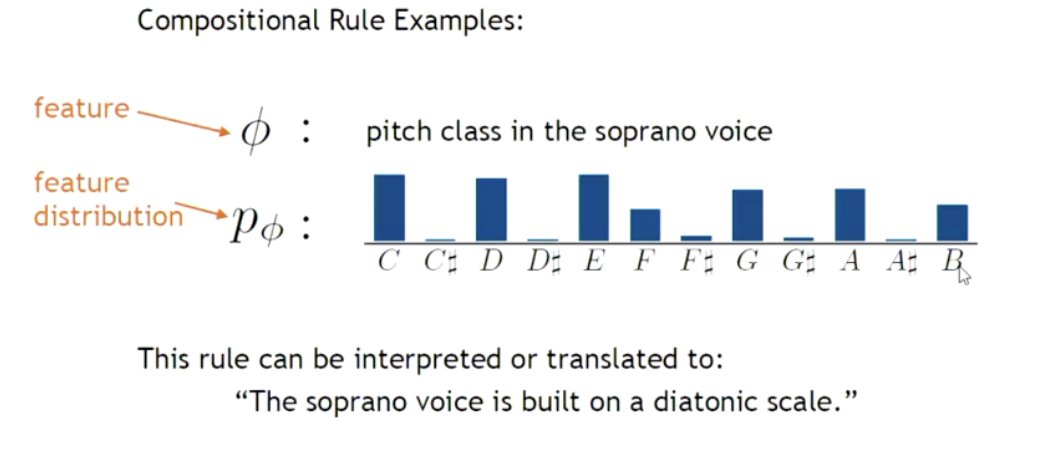
\includegraphics[width=\textwidth]{FIGS/rule1.png}
\caption{simple pitch class in soprano voice. Just C,D,E,F,G,A,B notes, without any sharps}
\label{fig:ai1}
\end{figure}

\subsubsection{Hierarchical concept learning}
\begin{figure}[!ht]
\centering
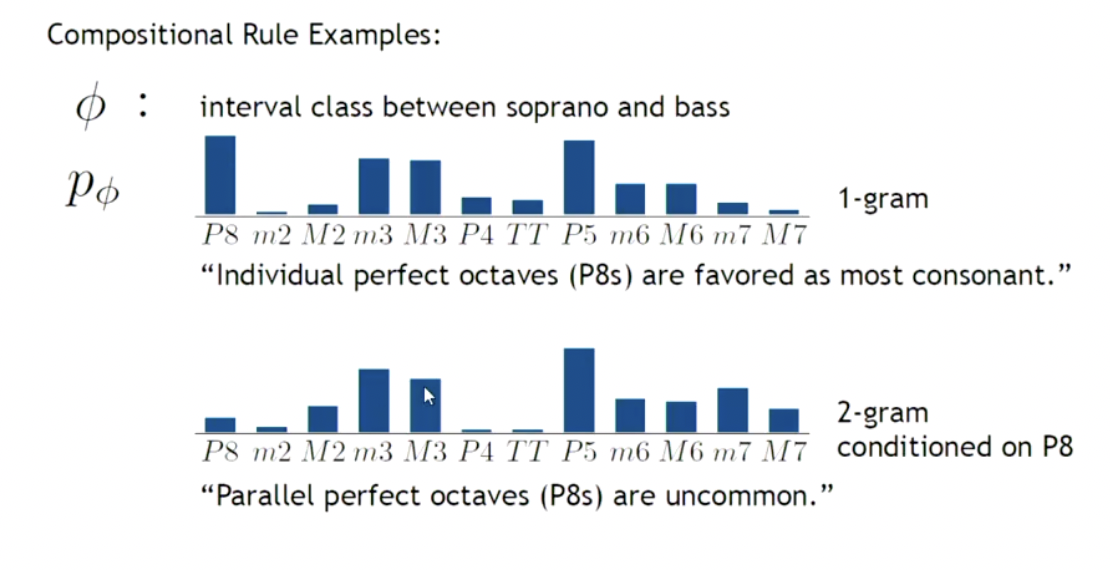
\includegraphics[width=\textwidth]{FIGS/rule2.png}
\caption{some composition rules as shown in the picture}
\label{fig:ai2}
\end{figure}

One way to prove that such rule is obvious to people is that we give an assignment that contains 25 rules(see the left figure in the figure~\ref{fig:ai3}) to students in CS and music class where most students are freshmen with limited knowledge in the area. After they finish the assignment, researchers find out the results in the right figure below. As we can see, 3 people get a perfect score and most students who finish the assignment get a score between 40 and 50, indicating that such rules are obvious to humans and interpretable. 
This form of compositional rules is in fact human-interpretable.

\begin{figure}[!ht]
\centering
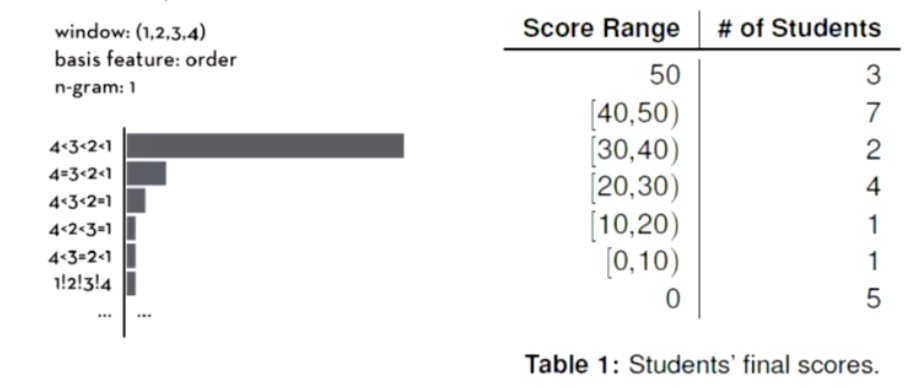
\includegraphics[width=\textwidth]{FIGS/rule3.png}
\caption{example of rules students get and the score they get in the assignment}
\label{fig:ai3}
\end{figure}


\section{Artificial Intelligence Creativity and \\Interpretability}
Nowadays, artificial intelligence (AI) starts to play a more and more important role in the creativity process, which is often thought of as the pinnacle of human achievement. 
Explainability on how creative AI is working, whether to engender trust, enable action, provide a basis for evaluation, or for intrinsic reasons is receiving broad attention in the AI community. 
Explainability is infinitely variable and there can be many valid explanations for given phenomena, particularly the inscrutability and non-intuitiveness. 
Inscrutability is when AI models available for direct inspection may defy
understanding due to their complexity; 
non-intuitiveness is when AI models are based on statistical relationships that defy human intuition even when they may be understandable.
Especially, interpretability for generative and creative models is critical as they are becoming widely used in many application domains, ranging from engineering, design and science, to the arts.
As shown in Fig.\ref{fig:ai}, as for explainability in generative algorithms, it's believed there can be a virtuous interaction among research in creative AI and explainable AI (XAI), all while interacting with human experts. 
In particular, this is the case when considering different kinds of creativity—combinatorial (which brings existing ideas together in new ways), exploratory (which expands the conceptual space), 
or transformational (which requires a completely new representation of conceptual domains)—and when considering a variety of explainability techniques, whether post-hoc or intrinsic. 
Notably, one may develop explanation-guided AI creations as well as more robust AI explanations. 
Moreover, when interacting with human experts, the result may be a better human–AI creative collaborations as well as better human-interpretable and trustworthy knowledge discovery.
    
\begin{figure}[!ht]
\centering
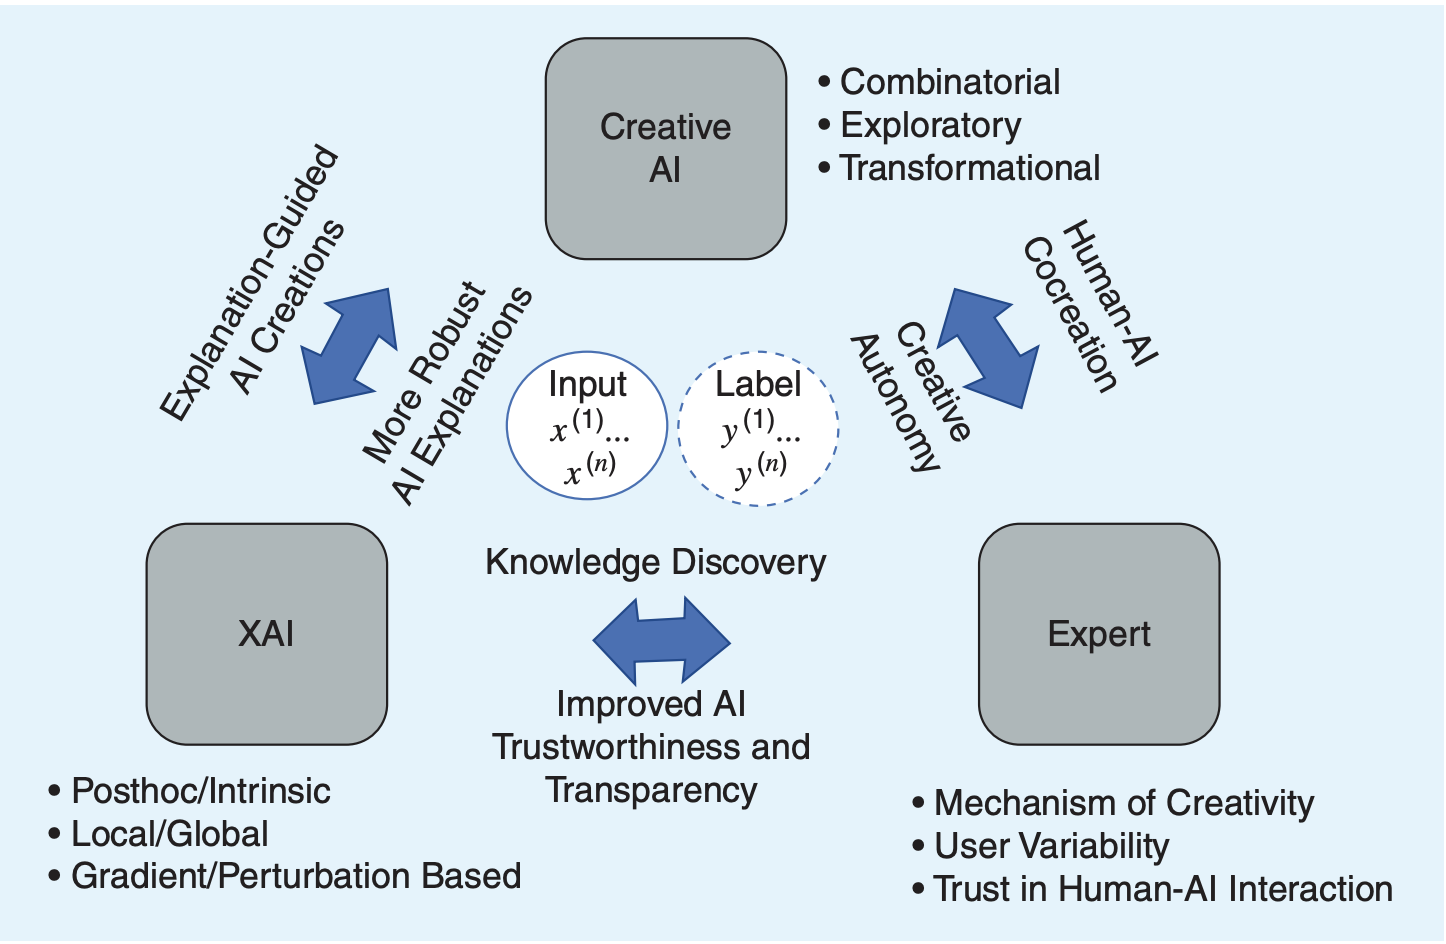
\includegraphics[width=\textwidth]{FIGS/ai_improve.png}
\caption{The expected improvements due to pursuing research at the intersection of creative AI, XAI and huamn-AI interaction (source: Payel \etal, 2022\cite{b1})}
\label{fig:ai}
\end{figure}



\subsection{Explaining Creative Artifacts}
With AI models becoming more complex and inscrutable, interpretable or XAI models are receiving broad attention. 
Generating explanations for black-box AI models is important, but assessing those explanations is challenging.
On one hand, it is not well defined how one should accurately account for the subjective variability in user perception of AI explanations. 
On the other hand, user perception can vary with the type of explanations provided. 

Most previous work in interpretable and explainable AI (XAI) has focused on decisions and predictions, that is, explanation of input-output mapping such as how do the given settings lead to given outputs. 
However, explaining the generated artifacts or the model itself of a generative AI framework has more challenges than the typical XAI paradigm for explaining predictive models. 
This is because the data distribution shift among training samples and generated artifacts often make explanations more difficult.
Methods for explainability of both the generative/creative algorithms or the ideas and artifacts they produce are considered and investigated. 
For the explanation of generative models, posthoc techniques (including visualizations) have been developed to interpret the generated outputs and have been applied to a variety of input modalities including images, natural languages, and tabular data. 
In addition, attention mechanisms\cite{b2} have played a major role in natural language modeling and generation, while the intermediate representations of these attention modules have been investigated for explaining the reasoning for a model's behavior. 

\subsection{Model agnostic interpretation}
Instead, another mode of explanation for the generated things is to address the artifacts where the generative models or algorithms are agnostic to the human. 
That means performing a model-agnostic interpretation of creative artifacts without considering how they are produced. 
The goal is to provide reasonable explanations for the generated data to the human rather than ensuring the explanation is absolutely authentic. 

Combinatorial and compositional creativity, the generation of unfamiliar combinations of familiar ideas, is the typical kind of creativity performed by people and also pursued by computational creativity systems, whether implicitly or through the explicit combining of parts. 
Although products of such creativity are interpretable for humans, their process may be inscrutable. 
An explanatory process is as important as the product for human understanding, especially when considering social creativity. 
For the explanation of this kind of creative artifact, One idea is to treat the explanatory process as an inverse problem, that is, an inverse problem formulation of going from a combinatorial artifact back to the human-like process that generates it without knowing the actual underlying algorithm. 

\subsubsection{Association chain}
The insights from human behavior science show that the human process of creativity is largely through associative chains. 
Human creativity processes are often thought of as forming associative elements into new combinations that either meet specified requirements or are in some way useful. 
Therefore, the artifacts explanation can be considered using the associated chain like what human creativity works. 

To find associated chains that use nearby associations, one can develop a traveling salesperson problem (TSP) formulation within knowledge graphs, where the modes are components and edges are associations. 
It's a kind of knowledge graph-based interpretation.
Tours, paths, and other combinatorial structures within the knowledge graphs are then possible explanations. 
The nearby associations are easier for people to understand.
In this sense, the explanation is the opposite of creativity.

\subsubsection{TSP formulation}
TSP consists of a salesman and a set of cities where the salesman has to visit each city starting from a certain city and returning to the same one. The challenge of the problem is to minimize the total length of the traveling length.  
It's NP-complete problem that can be modeled as an undirected weighted graph, as shown in Fig.\ref{fig:tsp}, where the cities are the graph's vertices, paths are the graph's edges, and a path's distance is the edge's weight. 
% Theoretically, it can be described as follows:
% $TSP=\{(G, f, t)\}$, where $G=(V, E)$ a complete graph with $V$ vertices and $E$ edges; $f$ is a function that finds the paths $Z$ from the space $V\times V$; $t\in Z$ is the pre-defined cost, $G$ is a graph that contains a traveling salesman tour with cost that does not exceed t. 

\begin{figure}[htbp]
\centering
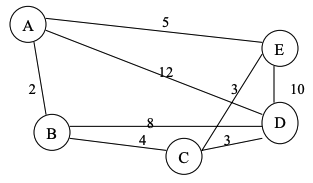
\includegraphics[width=0.6\textwidth]{FIGS/tsp-graph.png}
\caption{An Undirected weighted graph for TSP}
\label{fig:tsp}
\end{figure}

\subsubsection{Explanation examples with TSP formulation}
\textbf{Example 1}: The culinary recipe of a new spice mixture that can be used for pastries: thyme, clove, tangerine peel oil, French lavender, and lavender flower.

In this case, the shared flavor compound network proposed by Ahn \etal\cite{b3} provides the knowledge graph which can be used for explanations via flavor pairing hypothesis in culinary science. 
For the recipe in the example, the sub-graph with these components is extracted from the flavor compound knowledge graph, as shown in Fig.\ref{fl-tsp}. 
Within the sub-graph, two best TSP paths could be identified where edge weights are the number of shared flavor compounds (treated as strength of association). 
These two paths are the association chains, either "Clove$\rightarrow$Lavender Flower$\rightarrow$French Lavender$\rightarrow$Thyme$\rightarrow$ Tangerine Peel Oil" shown in the purple path or "Tangerine Peel Oil $\rightarrow$ Clove$\rightarrow$ Thyme $\rightarrow$ Lavender Flower $\rightarrow$ French Lavender" shown in the brown path. 
These TSP paths might provide the potential explanations that how the chief would come up with this recipe. 


\begin{figure}[htbp]
\centering
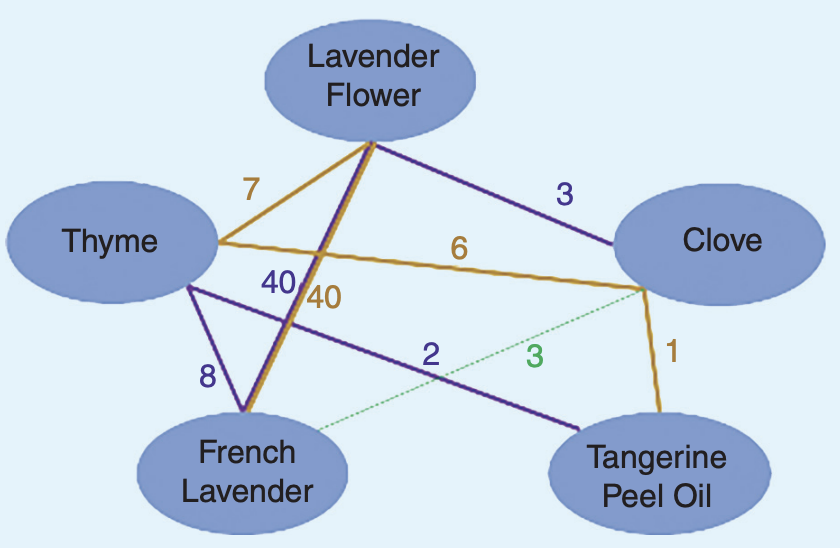
\includegraphics[width=0.6\textwidth]{FIGS/flavor_tsp.png}
\caption{A novel spice mixture explanation based on TSP. Explaining a novel spice mixture based on the number of shared flavor compounds (more is a stronger association), where two Hamiltonian paths are highlighted in purple and brown; and an unused edge is in green. Source: Payel \etal, 2022\cite{b1}}
\label{fl-tsp}
\end{figure}

\vspace{0.5cm}
\noindent\textbf{Example 2}: An English sentence: “After hearing the music, I woke up in the morning and opened my eyes, after which I had breakfast at the kitchen table.”

In this example, ConceptNet proposed by Liu \etal \cite{b4}is used as the 
knowledge graph, which represents natural language concepts with relations represented using commonsense reasoning. 
As shown in Fig.~\ref{eng-tsp}, use concept extraction to obtain the sub-graph from the whole ConceptNet, representing the concept graph in the example sentence. 
Then a TSP path is identified as shown in the green path. Traversing the TSP tour, "Hear Music$\rightarrow$Open eyes$\rightarrow$Wake Up in Morning$\rightarrow$Breakfast$\rightarrow$Kitchen Table", yields this sentence. 
Notice that the TSP tour is not in the same order as the sentence syntax, but is governed by the strongest semantic relationships. 
The edge labels provide human-interpretable explanations, such as “waking up in the morning is motivated by the goal of breakfast” even though this isn’t really in the sentence. 

\begin{figure}[htbp]
\centering
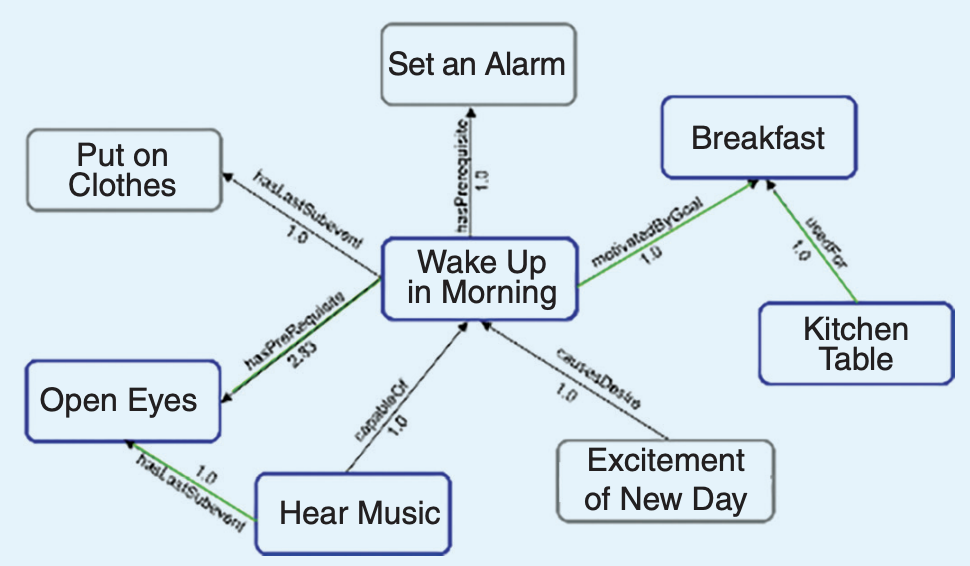
\includegraphics[width=0.6\textwidth]{FIGS/eng_tsp.png}
\caption{A English sentence explanation based on TSP. Explaining a novel English sentence, where a knowledge graph is denoted by blue nodes and corresponding edges among them, computed using ConceptNet (ignoring directionality, larger values are stronger associations). The gray nodes could have been used for augmentation if needed. The path highlighted in green is a traveling salesperson path. Source: Payel \etal, 2022\cite{b1}}
\label{eng-tsp}
\end{figure}

\vspace{0.5cm}
\noindent\textbf{Example 3}: A Hindi sentence that translates to “The old Indian government was the cause of other international governments unraveling.”

In this example, unlike the previous two examples which have knowledge graphs with explicit concepts and relationships, the Hindi or other low-resource languages don't have ConceptNet-like concept knowledge graphs. 
Instead of using the sub-graph from a known knowledge graph, the TSP path is identified on the word embedding space\cite{b5}, representing the implicit relationships from distances, as shown in Fig.~\ref{hindi-tsp}
 
\begin{figure}[htbp]
\centering
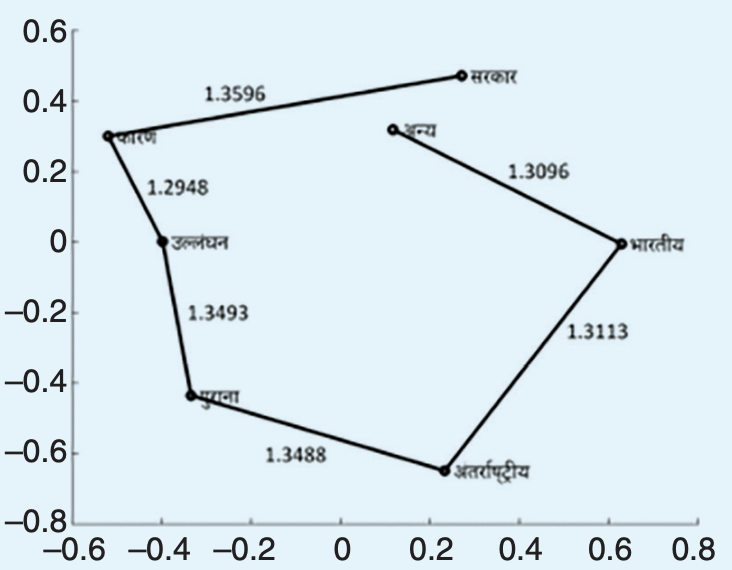
\includegraphics[width=0.6\textwidth]{FIGS/hindi_tsp.png}
\caption{A Hindi sentence explanation based on TSP. Explaining a novel Hindi sentence, computed using a pre-trained word embedding in a 2D principal component analysis basis. As this is a fully connected graph, we omit the unused edges in the traveling salesperson path. Source: Payel \etal, 2022\cite{b1}}
\label{hindi-tsp}
\end{figure}

\subsection{TSP path length as a measure of novelty}
In previous examples, rather than a statistical notion of novelty, a semantic notion of novelty based on explicit or implicit knowledge graphs is considered. 
It can be formalized as the \textit{TSP-novelty}. Considering a creative artifact $\alpha$ comprising components $\{x_1,..,x_n\}$ that has a corresponding sub-graph $\mathcal{G}$ of knowledge graph $\mathcal{K}$. Then the TSP-novelty of $\alpha$, $s_\mathcal{K}(\alpha)$, is defined to be $\mathbb{TSP}(\mathcal{G})$, where $\mathbb{TSP}(\cdot)$ is an operator for finding the traveling salesperson path length. 

Creative artifacts that connect semantically distant concepts seem to be very novel. 
Use computational geometry for the Euclidean TSP problem to characterize stochastic sampling-based creativity algorithms. Various generative algorithms like normalizing flows and VAEs can be thought of as stochastic sampling.
The following results can be obtained. 

\noindent\textit{Theorem 1}: Let $\{X_1,...,X_n\}$ be a set of independent identically distributed (i.i.d.) random variables in $\mathbb{R}^d$ with bounded support.
Then the length $L_n$ of the shortest TSP tour through the points $\{X_i\}$, satisfies: 

\begin{equation*}
    \cfrac{L_n}{n^{(d-1)/d}}\rightarrow\beta_d\int_{\mathbb{R}^d}f(x)^{(d-1)/d}dx
\end{equation*}


\noindent with probability 1 as $n\rightarrow \infty$, where $f(x)$ is the absolute continuous part of the distribution of the $\{X_i\}$, and $\beta_d$ is a constant that depends on $d$ but not on $f(x)$.
The choice of stochastic sampling distribution $f(x)$ in the creativity algorithm can directly control the traveling salesperson tour length in a given $d$-dimensional conceptual space. 
Taking $f(x)$ as the creativity algorithm, one can directly characterize the level of novelty it produces. 

Note that TSP tour length Ln is asymptotically, intimately tied to the Renyi entropy $H_\gamma(f(x))$ of the sampling distribution, where for $\gamma\in(0,1)$,

\begin{equation*}
    H_\gamma(f)=\cfrac{1}{1-\gamma}ln\int f(x)^\gamma(z)dz
\end{equation*}

\noindent and approaches the Shannon entropy as $\gamma\rightarrow 1$.

\noindent\textit{Theorem 2}: Let $\{X_1,...,X_n\}$ be a set of i.i.d.  variables in $R^d$ with bounded support. Let $L_n$ be the length of the shortest TSP tour through the points $\{Xi\}$. Then the following estimator for the Renyi entropy is asymptotically unbiased and almost surely consistent with the true Renyi entropy of $f(x)$.

\begin{equation*}
    \hat{H}_\gamma(f)(X)=\cfrac{1}{1-\gamma}(\cfrac{ln\ L_n}{n^\gamma}-ln\ \beta)
\end{equation*}
where $\gamma=(d-1)/d$ and $\beta$ is a fixed constant independent of $f(x)$.
The TSP tour length is asymptotically a simple function of the Renyi entropy of the stochastic sampling distribution, which approaches the Shannon entropy in high dimensions. So semantic novelty is intertwined with statistical novelty. 
In this case, these statistical measures of novelty, such as Shannon entropy and mutual information, are from a measure of novelty that emerges directly from explaining creative artifacts via associative chains. Thus the creativity algorithms can be designed directly using a measurement that emerges from explainability.


% \section*{References}
\begin{thebibliography}{00}
\bibitem{b1} Payel Das and Lav R. Varshney. "Explaining Artificial Intelligence Generation and Creativity: Human interpretability for novel ideas and artifacts", IEEE SIGNAL PROCESSING MAGAZINE, 1053-5888 (2022)
\bibitem{b2} Vig, Jesse. "A multiscale visualization of attention in the transformer model." arXiv preprint arXiv:1906.05714 (2019).
\bibitem{b3} Ahn, Yong-Yeol, et al. "Flavor network and the principles of food pairing." Scientific reports 1.1 (2011): 1-7.
\bibitem{b4} Liu, Hugo, and Push Singh. "ConceptNet—a practical commonsense reasoning tool-kit." BT technology journal 22.4 (2004): 211-226.
\bibitem{b5} Mikolov, Tomas, et al. "Distributed representations of words and phrases and their compositionality." Advances in neural information processing systems 26 (2013).
\bibitem{b6} "A Primer in BERTology: What We Know About How BERT Works | L3-AI 2021" https://www.youtube.com/watch?v=1aaWuAum5HY
\bibitem{b7} "BERTology meets Biology | Solving biological problems with Transformers" https://www.youtube.com/watch?v=pFf4PltQ9LY
\bibitem{b8} M. Mitchell, S. Wu, A. Zaldivar, P. Barnes, L. Vasserman, B. Hutchinson, E. Spitzer, I. D. Raji, and T. Gebru, "Model Cards for Model Reporting," in Proc. Conf. Fairness, Accountability, and Transparency (FAT* '19), pp. 220-229, Jan. 2019.
\bibitem{b9} M. Arnold, R. K. E. Bellamy, M. Hind, S. Houde, S. Mehta, A. Mojsilović, R. Nair, K. Natesan Ramamurthy, A. Olteanu, D. Piorkowski, D. Reimer, J. Richards, J. Tsay, and K. R. Varshney, "FactSheets: Increasing trust in AI services through supplier's declarations of conformity," IBM J. Res. Dev., vol. 63, no. 4/5, pp. 6:1-6:13, July-Sept. 2019.  
\bibitem{b10} "Devlin, Jacob et al. “BERT: Pre-training of Deep Bidirectional Transformers for Language Understanding.” ArXiv abs/1810.04805 (2019): n. pag."
\bibitem{b11} Koroteev, M. V. "BERT: a review of applications in natural language processing and understanding." arXiv preprint arXiv:2103.11943 (2021).
\bibitem{b12} Rogers, Anna, Olga Kovaleva, and Anna Rumshisky. "A primer in bertology: What we know about how bert works." Transactions of the Association for Computational Linguistics 8 (2020): 842-866.
\bibitem{b13} Haizi Yu and James Evans and Lav R. Varshney, "Information Lattice Learning", ICLR 2021, https://openreview.net/forum?id=SzjyTIc5qMP
\bibitem{b14} Cynthia Rudin, "Stop explaining black box machine learning models for high stakes decisions and use interpretable models instead", nature, https://www.nature.com/articles/s42256-019-0048-x
\bibitem{b15} Zihang Jiang, et al. "ConvBERT: Improving BERT with Span-based Dynamic Convolution", nips,  https://papers.nips.cc/paper/2020/file/96da2f590cd7246bbde0051047b0d6f7-Paper.pdf
\bibitem{b16} iren Chen, et al. "Improving BERT with Self-Supervised Attention", arXiv:2004.03808 [cs.CL]
\end{thebibliography}

\end{document}
